\section{Iteration \#1 -- Evaluation Framework and Baselines}

The first iteration was chosen to be two weeks long, instead of just one. This was to accommodate the extra work that would need to be done initially to lay the foundations that would be used to implement and evaluate the implementations. The objectives for this iteration were:
\begin{itemize}
	\item Design and implement a standard framework for evaluating index  in C++
	\item Implement evaluation baselines (Sequential Scan and Octree)
	\item Incorporate the School's implementation of the Pyramid Tree into framework
	\item Analyse performance of two baselines and the Pyramid Tree, evaluating their performance
\end{itemize}

\subsection{Data Generation}

TODO

\subsection{Evaluation Framework}

TODO: discuss design of this, what it does and WHY I decided to do it

TODO: what form an index structure takes -- i.e. its interface

\subsection{Baselines Implementations}

Sequential scan was implemented using \texttt{std::vector}, which is a dynamically resizeable array. Points insertion is $O(1)$ as they are to the end of the vector, deleting points results in a vector deletion, making it an $O(n)$ operation and point queries are $O(n)$, as the query iterates through the list until the given point is found or the end of the array is reached.

\subsection{Pyramid Tree}

TODO: how I got an implementation from a research fellow, etc. and modified it

TODO: added remove() and how I handled that

\subsection{Performance Analysis}

TODO: what I did for the performance analysis, what data I used, operation lists, etc.

TODO: compiler optimisation -- why I decided to not use -O1 

TODO: CPU and heap profiling

TODO: show all the graphs, tables, etc.

\begin{table}
	\centering
	\begin{tabular}{|l|l|l|l|l|l|l|l|l|}
		\hline
		\textbf{Structure} & \textbf{1D} & \textbf{2D} & \textbf{3D} & \textbf{5D} & \textbf{10D} & \textbf{50D} & \textbf{100D} & \textbf{200D} \\
		\hline
		\textbf{Sequential Scan} & 0 & 0 & 0 & 0 & 0 & 0 & 0 & 0 \\
		\textbf{Octree} & 0 & 0 & 0 & 0 & 0 & 0 & 0 & 0 \\
		\textbf{Pyramid Tree} & 0 & 0 & 0 & 0 & 0 & 0 & 0 & 0 \\
		\textbf{Pyramid Tree (No Defragmentation)} & 0 & 0 & 0 & 0 & 0 & 0 & 0 & 0 \\
		\hline
	\end{tabular}
	\caption{Execution Time of Structures for Uniform Randomly Generated Points with \texttt{-O1} Compiler Flag}
	\label{tab:perf1-randuniform-o1}
\end{table}

\begin{table}
	\centering
	\begin{tabular}{|l|l|l|l|l|l|l|l|l|}
		\hline
		\textbf{Structure} & \textbf{1D} & \textbf{2D} & \textbf{3D} & \textbf{5D} & \textbf{10D} & \textbf{50D} & \textbf{100D} & \textbf{200D} \\
		\hline
		\textbf{Sequential Scan} & 0 & 0 & 0 & 0 & 0 & 0 & 0 & 0 \\
		\textbf{Octree} & 0 & 0 & 0 & 0 & 0 & 0 & 0 & 0 \\
		\textbf{Pyramid Tree} & 0 & 0 & 0 & 0 & 0 & 0 & 0 & 0 \\
		\textbf{Pyramid Tree (No Defragmentation)} & 0 & 0 & 0 & 0 & 0 & 0 & 0 & 0 \\
		\hline
	\end{tabular}
	\caption{Execution Time of Structures for Uniform Randomly Generated Points with \texttt{-O3} Compiler Flag}
	\label{tab:perf1-randuniform-o3}
\end{table}
\begin{figure}
	\centering
	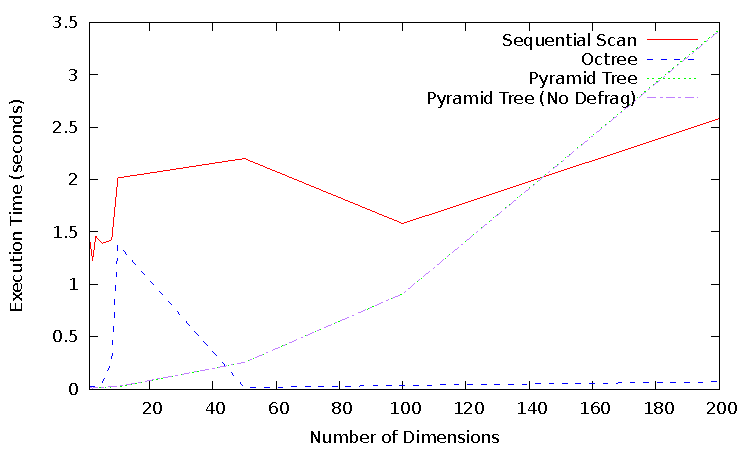
\includegraphics[scale=0.8]{../results/end_of_iteration1/all_insert_randuniform.pdf}
	\caption{\texttt{insert} Performance on Randomly Generated Uniformly Distributed Datasets}
	\label{fig:perf-1-allinsert}
\end{figure}

\begin{figure}
	\centering
	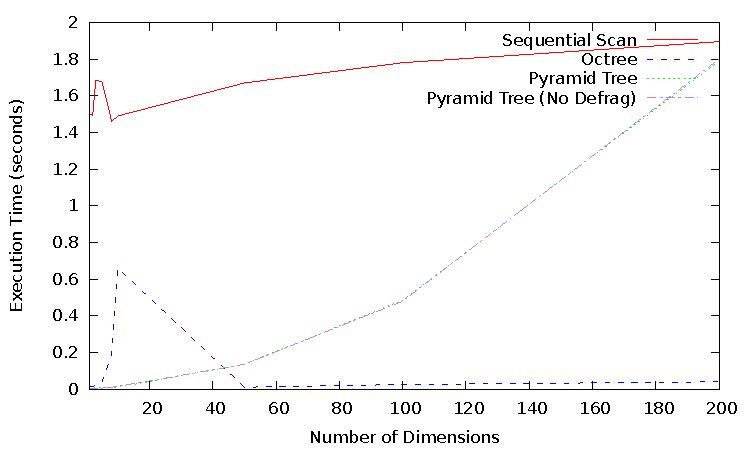
\includegraphics[scale=0.8]{../results/end_of_iteration1/all_pquery_randuniform.pdf}
	\caption{Point Query Performance on Randomly Generated Uniformly Distributed Datasets}
	\label{fig:perf-1-allpquery}
\end{figure}

\begin{figure}
	\centering
	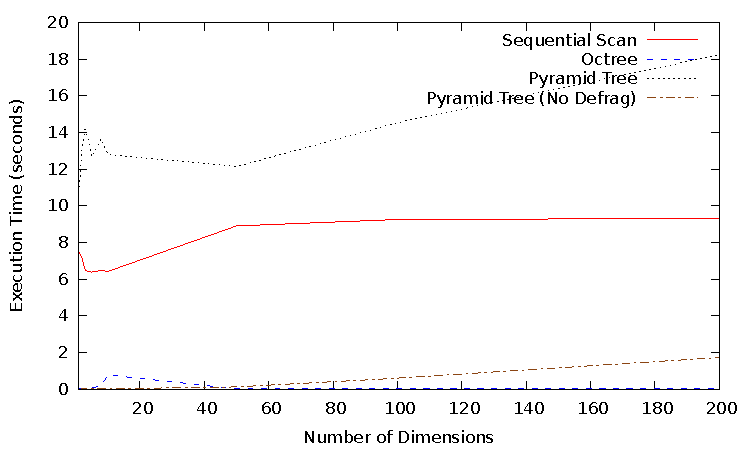
\includegraphics[scale=0.8]{../results/end_of_iteration1/all_delete_randuniform.pdf}
	\caption{\texttt{delete} Performance on Randomly Generated Uniformly Distributed Datasets}
	\label{fig:perf-1-alldelete}
\end{figure}

\subsection{Evaluation}

TODO: evaluate results in previous section

TODO state what was decided to do for next iteration (and why)
